% !TEX TS-program = xelatex
% !TEX encoding = UTF-8 Unicode

% This is a simple template for a LaTeX document using the "article" class.
% See "book", "report", "letter" for other types of document.

\documentclass[11pt]{article} % use larger type; default would be 10pt

\usepackage[utf8]{inputenc} % set input encoding (not needed with XeLaTeX)

%%% PAGE DIMENSIONS
\usepackage{geometry} % to change the page dimensions
\geometry{a4paper} % or letterpaper (US) or a5paper or....

\usepackage{graphicx} % support the \includegraphics command and options

% \usepackage[parfill]{parskip} % Activate to begin paragraphs with an empty line rather than an indent

%%% PACKAGES
\usepackage{paralist} % very flexible & customisable lists (eg. enumerate/compactitem, etc.)
\usepackage{verbatim} % adds environment for commenting out blocks of text & for better verbatim
\usepackage{listings} % for code blocks plus highlighting and stuff 
\usepackage[dvipsnames]{xcolor} % for the colors
\usepackage{graphicx} % for includegraphics
\usepackage{float} % for the H float option
\usepackage{ulem} % for strikethrough
\usepackage[hidelinks]{hyperref} % for links


%%% SECTION TITLE APPEARANCE
\usepackage{sectsty}
\allsectionsfont{\sffamily\mdseries\upshape} % (See the fntguide.pdf for font help)
% (This matches ConTeXt defaults)

% Dashes instead of dots for compactitem
\renewcommand\labelitemi{-}

%%% CODE STYLE
\lstdefinestyle{codestyle}{
	commentstyle=\color{Gray},
	keywordstyle=\color{RoyalBlue},
	numberstyle=\tiny\color{BrickRed},
	stringstyle=\color{ForestGreen},
	basicstyle=\ttfamily\footnotesize\bfseries,
	breakatwhitespace=false,
	breaklines=true,
	keepspaces=true,
	showspaces=false,
	showstringspaces=false,
	showtabs=false,
	tabsize=4
}
\lstset{style=codestyle}

%%% END Article customizations

\title{LarmLarms v1.0 Proposed Changes}
\author{}
% \date{} % Activate to display a given date or no date (if empty),
         % otherwise the current date is printed 

\begin{document}
\maketitle

\tableofcontents
\newpage

The proposed changes are mostly adding new features to the alarm app, but one change aims to reduce the features present in the app. Pretty much all of the screens would be changed in some way.

\section{Reducing Folder Ambiguity}
\label{sec:noOpenFolders}
We want to remove the ability for users to look at all folders at once. It's not used extensively, and creates confusion regarding which alarms are in which folders. While it's possible to make them more distinct, with the limited horizontal room of the mobile format, it's difficult to use the usual indenting to signify this. Instead, users will have to navigate to the desired folder to view alarms and folders within, truly integrating the tree structure of the folder system into the way alarms are presented.

\subsection{Code Simplification}
\label{sec:folderSimple}
This change would greatly simplify the code for folders and should reduce the number of things we need to store per folder. The lookup tables are completely unnecessary to connect \verb|RecyclerView| indices with actual alarms and folders. Every folder only shows immediate children, so the indices from the recycler view can be used to directly access the items in \verb|items|.

Open and closed folders no longer matter (and neither do the indents that helped to signify them) because there's only ever one folder being shown at a time. This would also solve the issue with small folder buttons within the larger item button doing different things, but would require some changes to recycler view items.

\subsection{Folder View}
This change also creates the need for a new activity which displays every item within a folder. Because it displays some different material, this activity would be separate from \verb|MainActivity|, and should always come with a folder attached in the \verb|Intent| (otherwise just exit). It would use the \verb|RecyclerView| that was originally only being used by the main activity. For the moment, there are very few customizable things about folders (name and location in the tree), so keeping all of them within this folder view activity is actually feasible. The main advantage of keeping the dedicated editor, though, is the ability to revert changes and ensuring fewer complications with adding any future folder customizations. 

\begin{figure}[h]
	\centering
	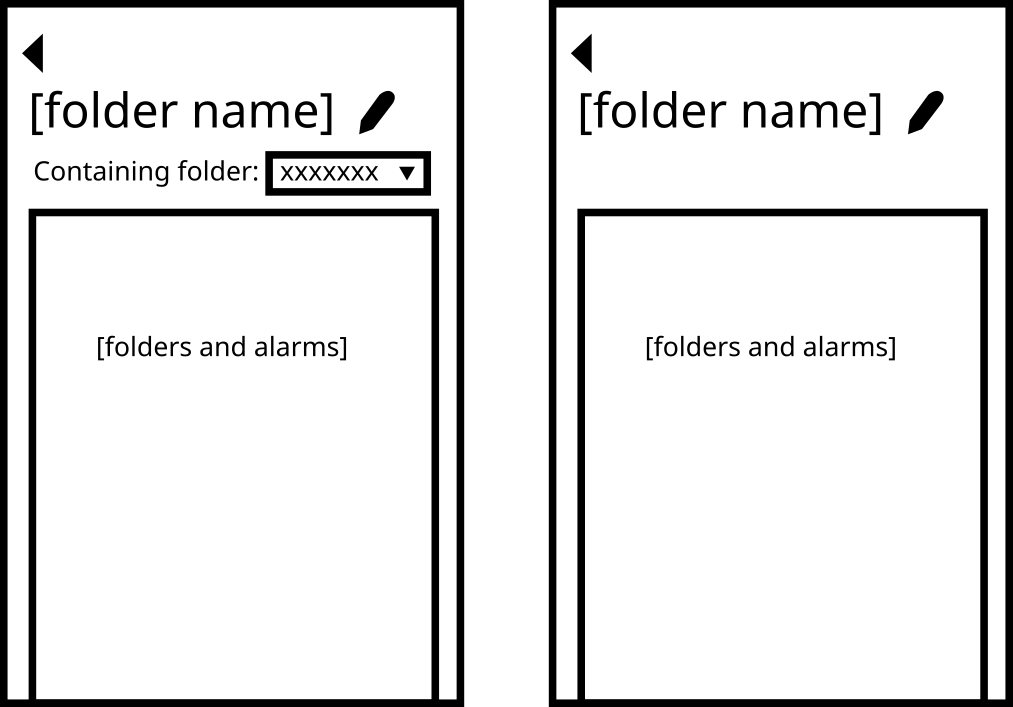
\includegraphics[scale=0.5]{possible folder view layout.png}
	\caption{Two possible layouts for the new folder view activity.}
\end{figure}

Users would be able to navigate to this new activity by single tapping the folder. This differs from the single tap of an alarm, but should be more intuitive because usually when clicking on a folder, users would expect to open the folder instead of edit it, reducing confusion. 

Each subsequent instance of the activity should also add to the activity stack. This allows users to return to parent folders when they're done viewing or editing the current folder. It shouldn't be possible to navigate to the folder view without starting from the root folder, so there should always be another activity before any folder view activity. 

\section{Default Alarms}
\label{sec:defaultAlarms}
Default alarms are what alarms are based off of when they're first created, and are bound to specific folders (including the root folder). If fields are left blank, it's assumed that they're inherited from their parent.

\subsection{Visibility in Folder View}
While the folders are usually sorted first by type (folders first), then alphabetically (then by ring type and time), the default alarm should always be at the top of the list. Since it's at the very top, transforming the \verb|RecyclerView| index into a \verb|items| index is simply subtracting 1. The fact that it's above all of the folders should also make it more clear to users that this is a special alarm, separate from the other ones.

\subsection{Default Alarm Storage}
Since default alarms are a folder-based feature, it should be stored with the folder it's associated with. While it's similar to a normal alarm, it doesn't have certain fields (such as an ID of its own or a ring time) and has the possiblity of blank fields as well to indicate inheritance. For this reason, adding it as part of the folder string structure makes sense. See sec. \ref{sec:folderChanges} to see all changes to the folder edit string.

\subsection{A New Editor}
We could've use the normal alarm editor to edit default alarms instead, but inheritance of the parent default alarms would've been a problem. How would users denote that they want inheritance from the parent folder? Without significant changes to the editor at startup, which would likely reduce performance, this wouldn't be possible. The user also shouldn't be able to enter things like name or ring time data, since none of that is stored (or makes sense for a template), so those fields would also need to be programmatically deleted. Because of this, a completely separate editor would be a better option.

To ensure it's intuitive for the user, the default alarm editor should look as much like the normal alarm editor as possible. The first thing should be the repeat type data, then ringtone, then volume and vibrate. However, if the repeat type usually has a date or time picker to indicate ring time, they shouldn't be present here. To make it completely clear this is a special alarm, we could also add also keep the alarm name text box but make it purely for show (to ensure users know this is distinct from a regular alarm). To denote inheritance, every field should have a checkbox next to it to enable or disable the option. When disabled, the default alarm won't change that field's data from its parent. Of course, if the alarm name text box is included, there shouldn't be a checkbox for it.

When attempting to open the activity, this editor could be used in conjunction with an explicit \verb|Intent| to open the activity, with the folder's edit string being added as data. 

Since this editor would be separate from the normal alarm editor, it would also make sense to separate the folder editor, since it really doesn't need to be packaged in a single class with the alarm editor, either. 

\subsection{Using Default Alarms}
A new method must be introduced in the \verb|AlarmGroup| class which creates a default alarm string when the user wants to create a new alarm. We can define a new format that follows the current default alarm format that can be added as data to the intents carrying the \verb|ACTION_CREATE_ALARM| action. To make this as simple as possible, we can simply apply all fields directly to the editor when they're passed in, instead of attempting to box them into an \verb|Alarm| where many junk fields could introduce clutter. The proposed string format is explained in sec. \ref{sec:defAlarmString}. To differentiate them from an actual alarm, it should be included in the extras with a different key (like \verb|EXTRA_DEFAULT_ALARM|).

\section{Item Duplication}
\label{sec:itemCopying}
In the case that a user has an alarm or folder they want to copy and edit, they should be able to long click on the item they want to copy and copy it from the dialog that pops up. Finally, it won't be just one item in the dialog. It could be a setting to immediately edit the new copy or not, and the default should be not to immediately edit. 

For the naming system, the first copy should tack on `` copy'' to the end of the name and every subsequent copy should add a number (starting at 2 and incrementing from there). To stay in line with user expectations, folder duplicates should be deep copies (have to recursively copy everything inside it as well). 

\section{Vacation Mode}
\label{sec:vacationMode}
Vacation mode is a feature for folders and recurring alarms. It shouldn't be possible to add a vacation mode for one-time alarms, because that doesn't really make sense, and folder vacation mode should only affect recurring alarms within itself. 

Because vacations should be able to be scheduled ahead of time, it requires both a beginning and ending date. It doesn't seem necessary to add any more granularity than days, and would only promote clutter and overwhelming numbers of options. The beginning and ending dates should default to the current date, so that if the user wants the vacation to start immediately, they only have to change one date, and both dates should be inclusive. These changes must be stored in the alarm and folder data itself, outlined in sec. \ref{sec:alarmChanges} and \ref{sec:folderChanges}.

\subsection{Adding/Editing Vacation Mode}
This is another function that should be accessible through long clicking an item. It should only show up if the item is either a folder or a recurring alarm, and should change based on whether vacation mode is already set for this item (change it from ``add'' to ``edit''). Once the option is clicked to add/edit a vacation mode, a new dialog should pop up with two dates (fig. \ref{fig:vacationAdd}).

\begin{figure}[h]
	\centering
	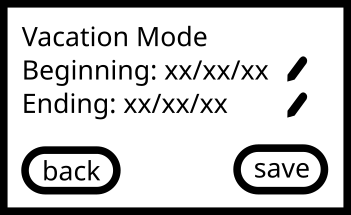
\includegraphics[scale=0.5]{vacation mode add dialog.png}
	\caption{Possible add dialog.}
	\label{fig:vacationAdd}
\end{figure}

\subsection{Editing Items with an Active Vacation Mode}
For folders, vacation mode should be completely unaffected no matter what the user changes. However, for alarms, vacation mode can be removed if the alarm is changed to a one-time alarm. Otherwise, it should remain intact. 

\subsection{Deleting Vacation Mode}
Once an item gain a vacation mode, a new option should appear in the long tap menu to delete it. When it gets deleted, both the start and end dates can be set to 0 to ensure both are in the past.

\section{Customizable Snoozing}
\label{sec:customSnoozing}
A new feature with alarms: to be able to customize how long snoozes are. This mainly shows up on the ring time screen as a number entry with plus or minus signs next to it to increment and decrement the number of minutes. The entire layout should be above the snooze button (right below the alarm name). The default snooze time should be customizable via slider in the alarm editor. 

This requires some changes in how we currently handle snoozing. If the amount of time this is snoozed is variable, then instead we must store the amount of time the alarm has been snoozed for. This also supports the next ring time being based on the current time (instead of being based on the time the alarm started ringing, which might be far into the past). 

\section{Automatic Folder Activation}
\label{sec:autoFolderActivation}
This is a new setting that can activate all containing folders when a new alarm (not folder) is set. It should also activate when users activate any item. 

\subsection{Parent Child Relationships}
\label{sec:folderRelations}
With this change, we should also consider how a folder is stored in relation to the rest of the structure. The parent of the current item should be cached just as its children are. This would make the folder structure similar to both a doubly linked list and a tree, and would simplify going up to parent folders to check for activation if necessary.

\section{Changes to String Storage}
\label{sec:stringChanges}
\subsection{Alarm}
\label{sec:alarmChanges}
All fields are required unless otherwise listed. New fields are bolded. 
\begin{table}[H]
	\centering
	\begin{tabular}{c|c}
		Field & Datatype \\ \hline
		id & \verb|int| \\
		name & \verb|string| \\
		is active & \verb|bool| \\
		repeat type & \verb|string| \\
		ring time & \verb|long| \\
		ringtone uri & \verb|string| (stringified URI) \\
		is snoozed & \verb|bool| \\
		number of snoozes & \verb|int| \\
		volume & \verb|int| \\
		vibrate & \verb|bool| \\
	\end{tabular}
	\caption{Revised alarm edit string format}
\end{table}

\subsection{AlarmGroup}
\label{sec:folderChanges}
All fields are required unless otherwise listed. New fields are bolded, and fields being removed are struck through.
\begin{table}[H]
	\centering
	\begin{tabular}{c|c}
		Field & Datatype \\ \hline
		id & \verb|int| \\
		name & \verb|string| \\
		is active & \verb|bool| \\
		\sout{is open} & \verb|bool| \\
		\textbf{default alarm (optional)} & \verb|string| (see sec. \ref{sec:defAlarmString}) \\
	\end{tabular}
	\caption{Revised folder edit string format}
\end{table}

If there is no default alarm, a trailing tab should still be present. 

\subsection{Default Alarm (new)}
\label{sec:defAlarmString}
All fields are required unless otherwise listed. All of this is new, so there's no bold or strikethrough to be seen here.
\begin{table}[H]
	\centering
	\begin{tabular}{c|c}
		Field & Datatype \\ \hline
		repeat type (optional) & \verb|string| \\
		ringtone uri (optional) & \verb|string| (stringified URI) \\
		volume (optional) & \verb|int| \\
		vibrate (optional) & \verb|bool| \\
		snooze length (optional) & \verb|int| \\
	\end{tabular}
	\caption{New default alarm string format}
\end{table}

Just as the alarm and folder strings are, the default alarm strings should also be separated by tabs. All fields are optional when in use, and the repeat type format follows the repeat type format for normal alarms. In the case that any field is blank, the tabs between the field should still be present to preserve order and show that the field is actually blank.

\section{Order of Changes}
To ensure the least amount of headache, we also aim to create an order to the changes. It reduces the number of times that edit or store strings change, so that validation functions should only need to be changed and tested once. It also 

\begin{compactenum}
	\item Change folders to a more tree-like structure and simplify the class (sec. \ref{sec:folderSimple} and \ref{sec:folderRelations}).
	\item Add the folder view activity and adapt all UI code to the new folder structure (sec. \ref{sec:noOpenFolders}). 
	\item Change all edit strings to the new format (sec. \ref{sec:stringChanges}). 
	\item Add default alarm functionality and change UI to match (sec. \ref{sec:defaultAlarms}).
	\item Add item duplication (sec. \ref{sec:itemCopying}).
	\item Add vacation mode (sec. \ref{sec:vacationMode}). 
	\item Add customizable snoozing (sec. \ref{sec:customSnoozing}).
	\item Add automatic folder activation (sec. \ref{sec:autoFolderActivation}).
\end{compactenum}

\end{document}
